\documentclass[10pt, oneside,spanish]{article}   	
\usepackage{geometry}
\usepackage{amsmath}
\geometry{a4paper}                   		
\usepackage[utf8]{inputenc}               	 
\usepackage{listings}	
\usepackage{tabu}


\usepackage{graphicx}												
\usepackage{amssymb}
\usepackage{authblk}
\usepackage{relsize}



\linespread{1.5}

\title{MKTG 212 - Case 5: Factor Analysis} \lstset{language=R}

\author[]{Juan Manubens}

\affil[]{University of Pennsylvania}
\renewcommand\Authands{, }
\date{}							
\begin{document}
\maketitle



\section{Ford KA Case}


\begin{itemize}
\item \textbf{[1a] Describe the small car market in France.  What are the major customer groups and what are their needs?  }
\end{itemize}

A “small car” is any car with less than 390 cm in length (excluding a few cars - these exceptions are classified as sports vehicles).  In France, the small car market is large, making up 43.7\% of the new cars sold in 1995 (as compared to in Europe overall, in which small cars only accounted for 32.2\% ).  In France, people who own small cars pay notably less tax on their cars than people who own larger cars.  Therefore, the small car market was more developed in France than in other European nations.  Manufacturers of small cars usually specialized in producing a certain subset of small car rather than an array of product offerings.  For example, luxury car companies such as Mercedes and BMW concentrated on advanced product features and quality, while other companies like PSA, Renault, and Fiat competed on price by realizing high volumes and therefore low manufacturing costs.

In the 1980's and early 1990's, a number of factors led to an increase in small cars' popularity in France.  Increased road congestion, difficulty parking in big cities, and high fuel prices made smaller, low-fuel cars more attractive to consumers.  Additionally, the number of working women increased, which meant that more women - who exhibited a general preference for small cars - were buying cars.  Average household size decreased to fewer than three members, which meant that more households could fit everyone in a smaller car.  This increased popularity led to increased competition within the small car market.  New models such as the \textit{Clio}, the \textit{Twingo}, the \textit{Punto} by Renault, among others, were launched in a period from 1990 through 1994, and existing models such as the \textit{Corsa} by Opel in 1992 and the \textit{Polo} by Volkswagen in 1994 were upgraded.  Car companies that had until this point focused solely on large cars began to move into the market.  This happened first with BMW’s 1994 acquisition of Rover, as it was based in part on the idea of owning Rover's small car line.  In 1997, Mercedes followed BMW into the market by launching the Mercedes \textit{A-Class}; the Smart car came soon afterwards.  In 1995, Renault owned the largest share of the French small car market at 36.6\%, followed by PSA with 26.1\%, the Italian company Fiat with 11.0\%, and Ford and and GM's German subsidiary Opel, both with 7.6\%.    

Traditionally, the European small car industry segmented the market into tiers based on size.  Because there was a strong correlation between the size of a car and its production cost – and therefore its price – the market was segmented by age and income.  Older, wealthier buyers and families purchased larger small cars, while younger, lower income buyers bought smaller small cars.  However, the market was changing rapidly, and consumer desires were becoming more varied.  Price was no longer the most important factor in a purchase decision.  Some customers looked for more safety features like airbags and an anti-lock brake system, space and functionality, comfort, or power steering.  Older purchasers often expected small car to have features similar to the large cars they were used to.  Four different types of small car emerged to serve four different consumer segments.  Category A small cars were practical "\textit{run-arounds}", were under 360 cm long, and made up 6\% of the French market.  Category B was divided into three subcategories.  The first was the Basic-B category, which exhibited trends always associated with small cars and comprised 40\% of the market.  There was also the Trend-B category (52\%), which flaunted better performance and more features, like equipment previously only offered in large cars.  Other-B was the remaining 2\% of the market and consisted of luxury and sports small cars.  The four main market segments were Middle-Aged Buyers, who needed safety, reliability, and value; Singles, who wanted individuality and personality; Families, who valued functionality, space, and reliability, and Women, who looked for value and a combination of all the other factors.       



\medskip


\pagebreak


\begin{itemize}
\item \textbf{[1b] Using the data from the customer survey, evaluate if demographic variables separate out “\textit{Ka} Choosers” and “\textit{Ka} Non-choosers”. How do you propose to address the people in the “middle”? Are your main findings the same with / without considering the middle group?}
\end{itemize}

\begin{center}
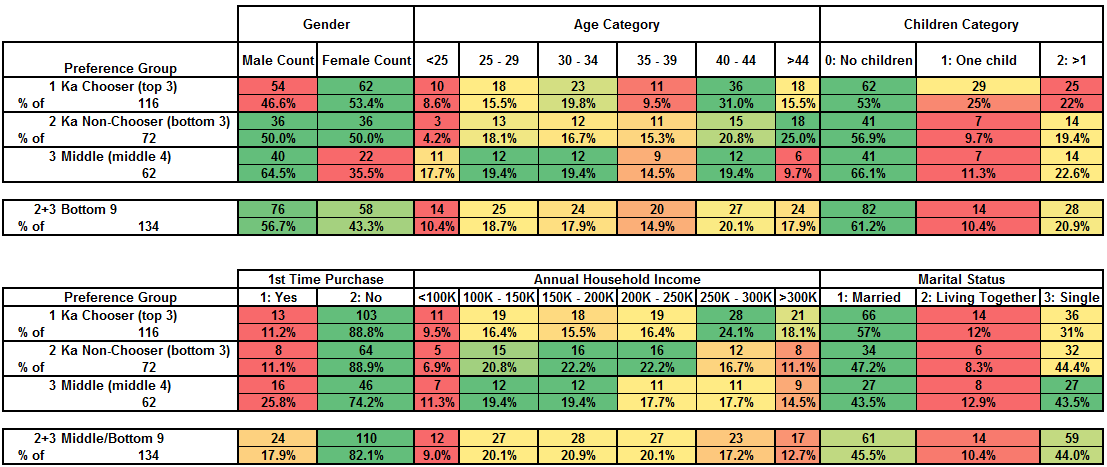
\includegraphics[width=15cm]{1b1.PNG}
\end{center}

We approached this in two different ways: (1) We ran a $k=2$ means clustering on the subset of the data containing only KA choosers and non-choosers (2) We examined the summary statistics of the demographic variables (see table above). The clustering was not very effective (it classified roughly $\approx 49.8 \%$ of the clusters correctly, or just as good as chance). Looking at the demographic variable summaries gives us a better picture: \textit{Ka} choosers, relative to non-choosers, are more likely to be female, older, less likely to have any children, and wealthier. \textbf{Nevertheless, once we include the middle 4 into the analysis, the biggest issue is that the data does not follow a linear trend as we go down the preference ranks, and the groups vary heavily in size.} The middle 4 preference group is more likely to be male, and relative to both choosers and non-choosers tend to be younger, less likely to to have kids, and less wealthy. 

Given that the demographic variables do not follow a linear trend, it seems incorrect to label the middle group as "the middle", and it is more useful and differentiating to either cluster preference groups 2 and 3 together, or to only compare and contrast choosers and non-choosers. However, blending non-choosers and the middle group, given the non-linear relationship described above, could be highly misleading.

\pagebreak


\begin{itemize}
\item \textbf{[1c] Goldfarb later claimed to identify four attitudinal segments from the survey: Freedom Lovers, Attention Seekers, Sensible Classics, and No-nonsense neutrals.  Using the data provided for this case (see Canvas for the Excel file), illustrate the process used for identifying the attitudinal segments. Answer the following using the customer survey data provided with the Ford \textit{Ka} Case. Using the 62 attitude questions as variables for segmentation:  }
	\begin{enumerate}
    \item \textbf{Identify the number of clusters.  How many customers belong to each cluster?}
    
   In order to make sense of the data we ran a factor analysis on the 62 questions; this analysis yielded 9 factors with Eigenvalues greater than 1. We loaded the survey questions on to these factors according to whichever of the nine factors had the highest loading (in absolute terms) respective to each of the 62 questions. This produced significant differences in terms of how many questions was loaded onto each factor; for example, 25 questions belong to Factor 1 while no questions had the highest absolute loading value with respect to Factor 9. (The attached back-up spreadsheet shows how the questions were allocated). 
   
   We decided to name the factors according to general themes. Factor 1 encompassed a wide range of questions so it was difficult to pinpoint, but most questions related to "Brand and Image" concerns. Factor 2 was primarily related to "Practicality". Factor 3 primarily encompasses "Idealistic and Socially Conscious" questions. And the majority of questions incorporated into Factor 4 addressed "Usage and Functionality". Factors 5-9 were generally very limited in the number of questions, so we decided to simply name them by their number.
   
   Based on these 9 new factors, we conducted a cluster analysis, which showed that three clusters were optimal. Nevertheless, we decided to use four in order to compare them to Goldfarb's four clusters, as per the case questions.  The number of customers per cluster is 77 for Cluster 1, 61 for Cluster 2, 80 for Cluster 3, and 32 for Cluster 4.
    
\pagebreak  
\item \textbf{Name the clusters using the difference in mean scores across the clusters on all 62 attitudinal questions.}
    
\begin{center}
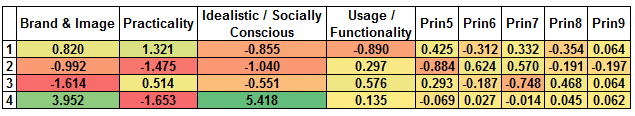
\includegraphics[width=13cm]{1c1.PNG}
\end{center}
    
Cluster 1 has a relative high score on the second Factor, "Practicality" while idealistic concerns ranked relative low in importance. An appropriate name could be "Practicality-Seekers", or perhaps "Sensible Classics"

Cluster 2 is relatively ambivalent and hard to distinguish from the other clusters. If anything, it is noteworthy that they have relatively low mean scores for the three factors (numbers 1-3) that are generally more important for the other clusters. They are mostly defined by their preference for functionality or perhaps Stability (inferable from their scores on factors 4 and 7). Thus, we have named them "Stability-Seekers".

Cluster 3 is also a fairly neutral cluster. They generally have intermediately high scores on "Practicality" and "Usage/Functionality" and low scores on "Brand and Image." Thus we think that "No-Nonsense Neutrals" is an appropriate name.

Cluster 4 has very high scores on the factors "Brand and Image" and "Idealistic and Socially Conscious" and comparatively much lower scores on "Practicality." This implies that they care more about appearance and social issues relative to the other clusters. We therefore think "Attention Seekers" is a reasonable name. 
        
    \item \textbf{Do you agree with Goldfarb’s naming of the four attitudinal segments as: Freedom Lovers, Attention Seekers, Sensible Classics, and No-nonsense neutrals? (Hint: you may want to think about factor analysis).}
    
 Generally, we think that the clusters are fairly similar.  We took on three of the four same names; the only difference is that we named one of the segments "Stability Seekers," while Goldfarb called it "Freedom Lovers."  We chose the label "Stability Seekers" because the answers this segment gave indicated a preference for a car that will drive them someplace and little care about anything else. 
 
 We primarily felt limited in our ability to compare the two sets of clusters in that clusters 1 and 4 were highly distinguishable, while clusters 2 and 3 did not really stand apart significantly. We believe this effect was exacerbated by the fact that factor 1 was so all-encompassing while some of the factors were very limited and at times appeared hard to generalize. 
    
    \item \textbf{Are there any differences among the four segments based on demographics?}
    
Regarding the purchaser's gender, only Stability Seekers are more female-heavy; the rest of the segments see more male purchasers (though the split appears close to 50/50 for all segments).  Age appears not to differ across segments, as all segments have an average age of about 37 for the purchaser.  In terms of marital status, all segments  have the largest portions of married customers, followed by single customers.  Few purchasers live with a non-spouse significant other.  The Stability Seekers segment stands out in that it the portions of married and single customers are almost equal.  In the other segments, the percentage of single customers is lower. Number of children is nearly equal for Sensible Classics and Stability Seekers (lower than for the other two segments),  and highest for No-Nonsense Neutrals.  The number of  customers for which it was their first time buying a car was highest  for Stability Seekers and lowest for Sensible Classics and Attention Seekers equally.  With respect to income, Attention Seekers  are largely concentrated in low and high income, with the lowest percentage of middle income among the segments.  In contrast, Sensible Classics are skewed toward middle income.  Both Stability Seekers and No-Nonsense Neutrals are mainly middle- to high-income.  

While there are observable differences in the demographic make-up of the different clusters, we generally found that these differences were relatively small. This implies that it makes sense to focus on customer segmentation along the lines of preferences rather than just demographic data as was done in the past. In other words, you cannot necessarily predict a customer's consumption preferences based on their gender, age or income level.
    
    \end{enumerate}
\end{itemize}

\pagebreak

\begin{itemize}
\item \textbf{[1d] What marketing strategy do you suggest for Ford \textit{Ka}?  }
\end{itemize}

The data suggests a few viable marketing strategies:

\begin{enumerate}
\item If Ford believes that the \textit{Ka} is most like to sell among low-income consumers, it makes sense to target the "Attention-Seekers" segment (cluster 4) -- 40\% of this cluster is in the bottom 2 income groups. As such, Ford might emphasize design, image and idealistic messages (e.g. fuel-usage) in its advertising. It seems the attention seekers want something that stands out, so it would be important to emphasize its unique features. Furthermore, we would suggest have a strong advertising campaign as soon as the Ka is released, as this segment will probably want to buy it as soon as it comes out and not many people own it yet.

\item If Ford believes the car will sell best to first-time buyers with no children it might consider instead targeting Cluster 2 ("Stability-Seekers"). As such it could advertise the car as a reliable, value-for-money option for new customers in the car market. They would focus on the tangible benefits of the car and how durable it is, to emphasize the value they gain for its price. This segment, as they are looking for a stable car, may also do more detailed research onto their other options, so it may be important to emphasize the benefits of the \textit{Ka} in comparison to other models or brands. 

\item Finally, the survey data analyzed in 1(b) suggests that a larger emphasis should be placed in targeting female consumers. Consequently, clusters with a higher proportion of women should be perceived as more valuable.
\end{enumerate}
In considering these options, Ford should also take into account how the existing cars on the market are perceived and make sure that it chooses a branding message that does not overlap too much with another car (or, if it does, ensure that the \textit{Ka} is competitive relatively speaking). It may also want to ensure that it does not cannibalize its sales for other models.  The company can use perceptual maps to accomplish this. 






\end{document}   
